\chapter*{Annexes}
\addcontentsline{toc}{chapter}{Annexes}
 
\section*{Page d'accueil}
Dans notre site nous avons un seul utilisateur qui est l'agent. Au lancement du site la page principale s'affichera avec la liste des avis avec les fonctionnalités du site.
\medskip

\begin{figure}[h!]
    \centering
    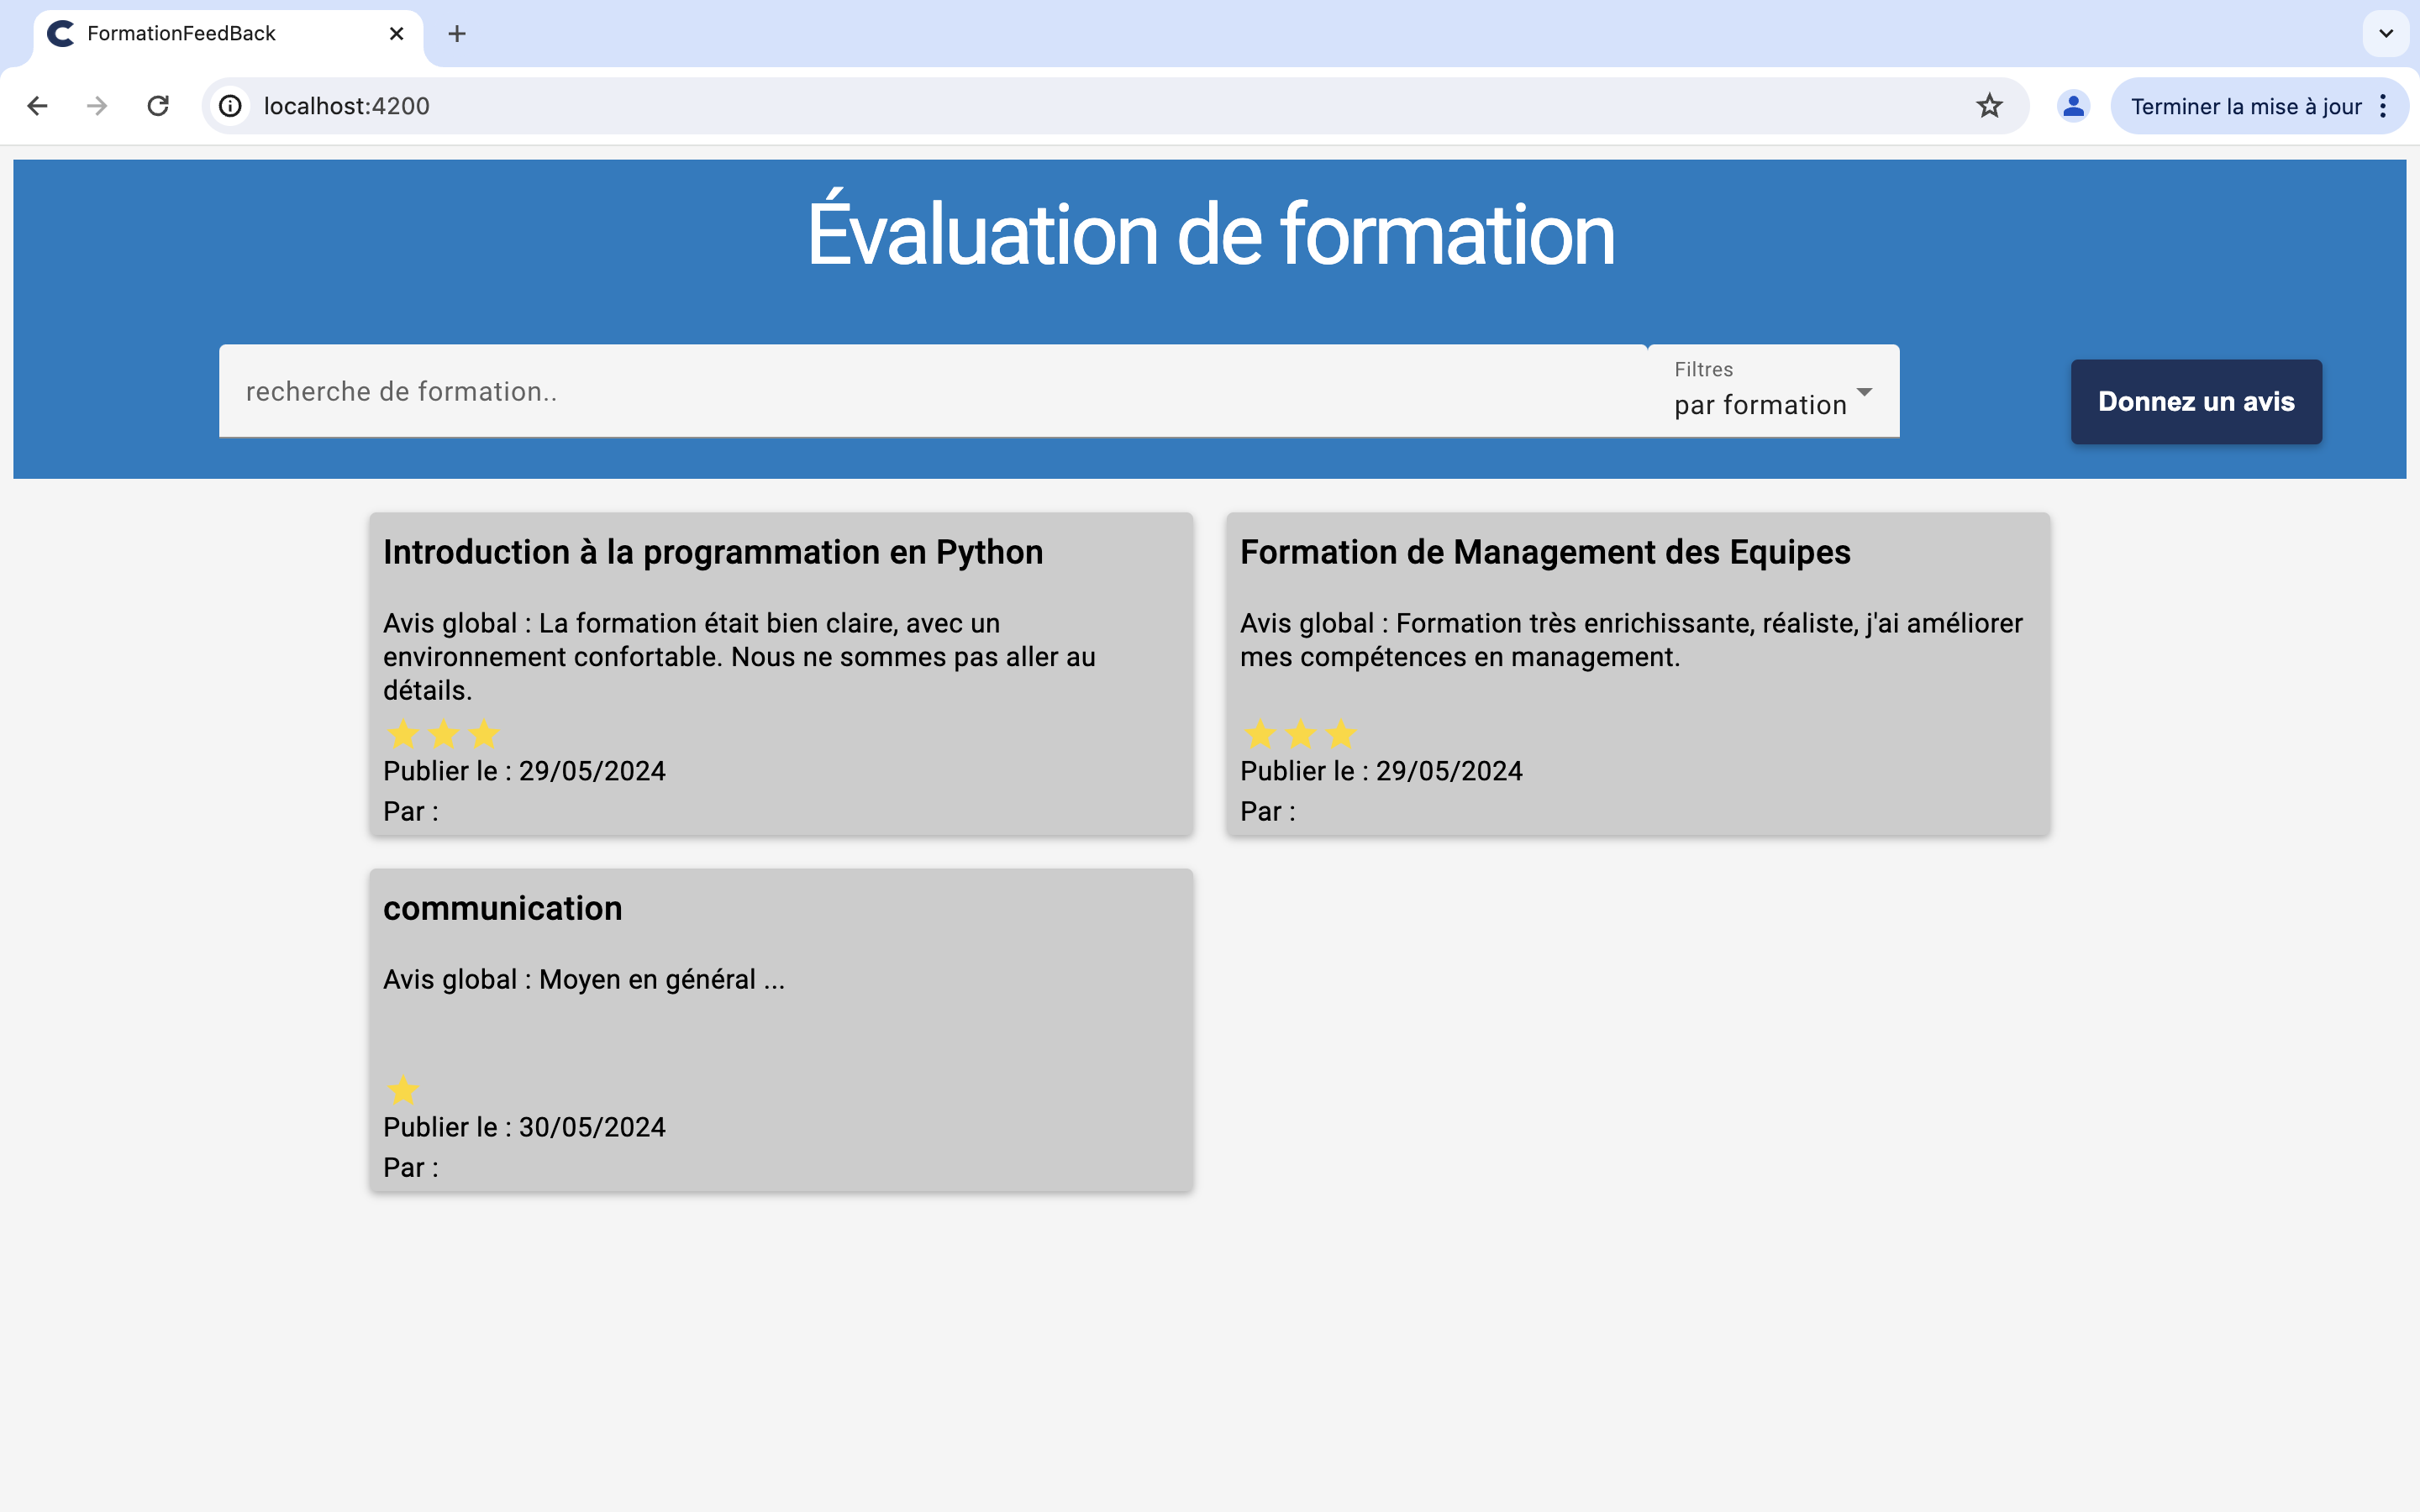
\includegraphics[width=1\textwidth]{images/fenetres/accueil.png}
    \caption{Page Principale}
\end{figure}

\newpage

\section*{Ajouter un avis}
Lorsque l'agents veut ajouter un avis sur une formation qu'il à suivi, il clique sur le bouton 'Donnez un avis', une fenêtre modale du formulaire s'ouvre, il remplit les champs nécessaires. 
\medskip

\begin{figure}[h!]
    \centering
    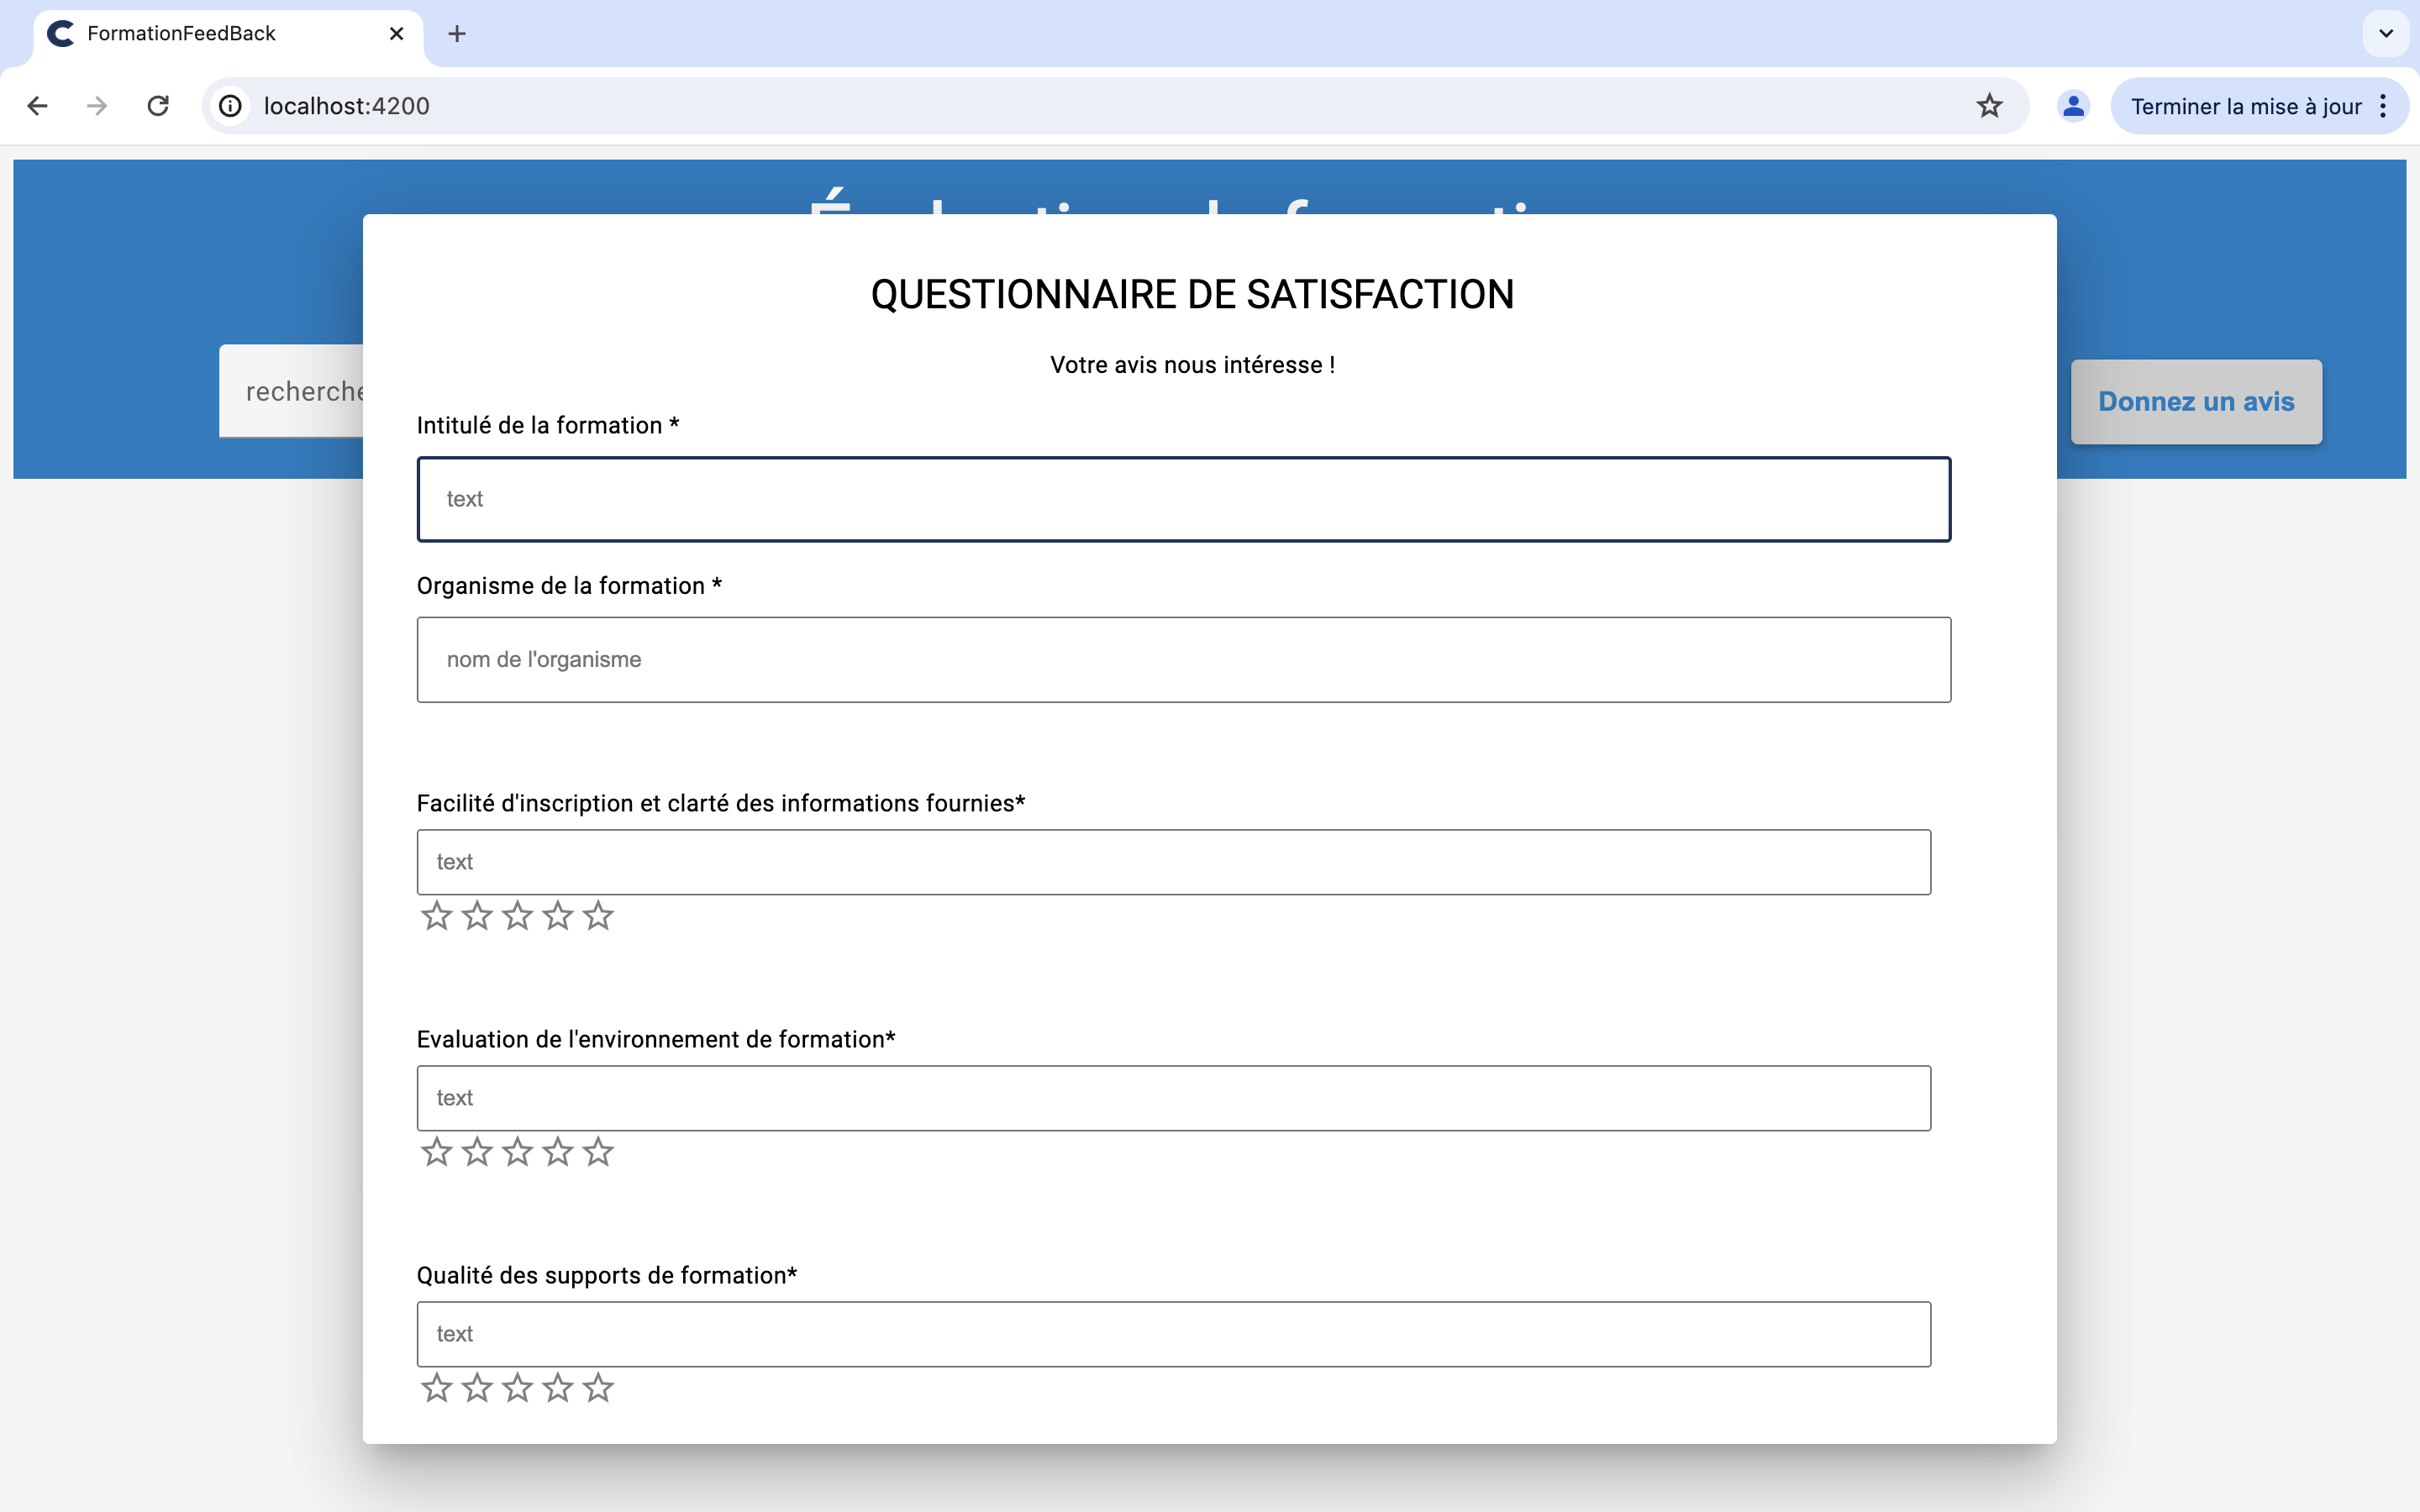
\includegraphics[width=1\textwidth]{images/fenetres/AjouterAvis.png}
    \caption{Formulaire d'ajout d'un avis}
\end{figure}

\newpage

\section*{Rechercher un avis}
On peut aussi rechercher un avis par des filtres, exemple mot clé où par formation les mieux notée.
\medskip

\begin{figure}[h!]
    \centering
    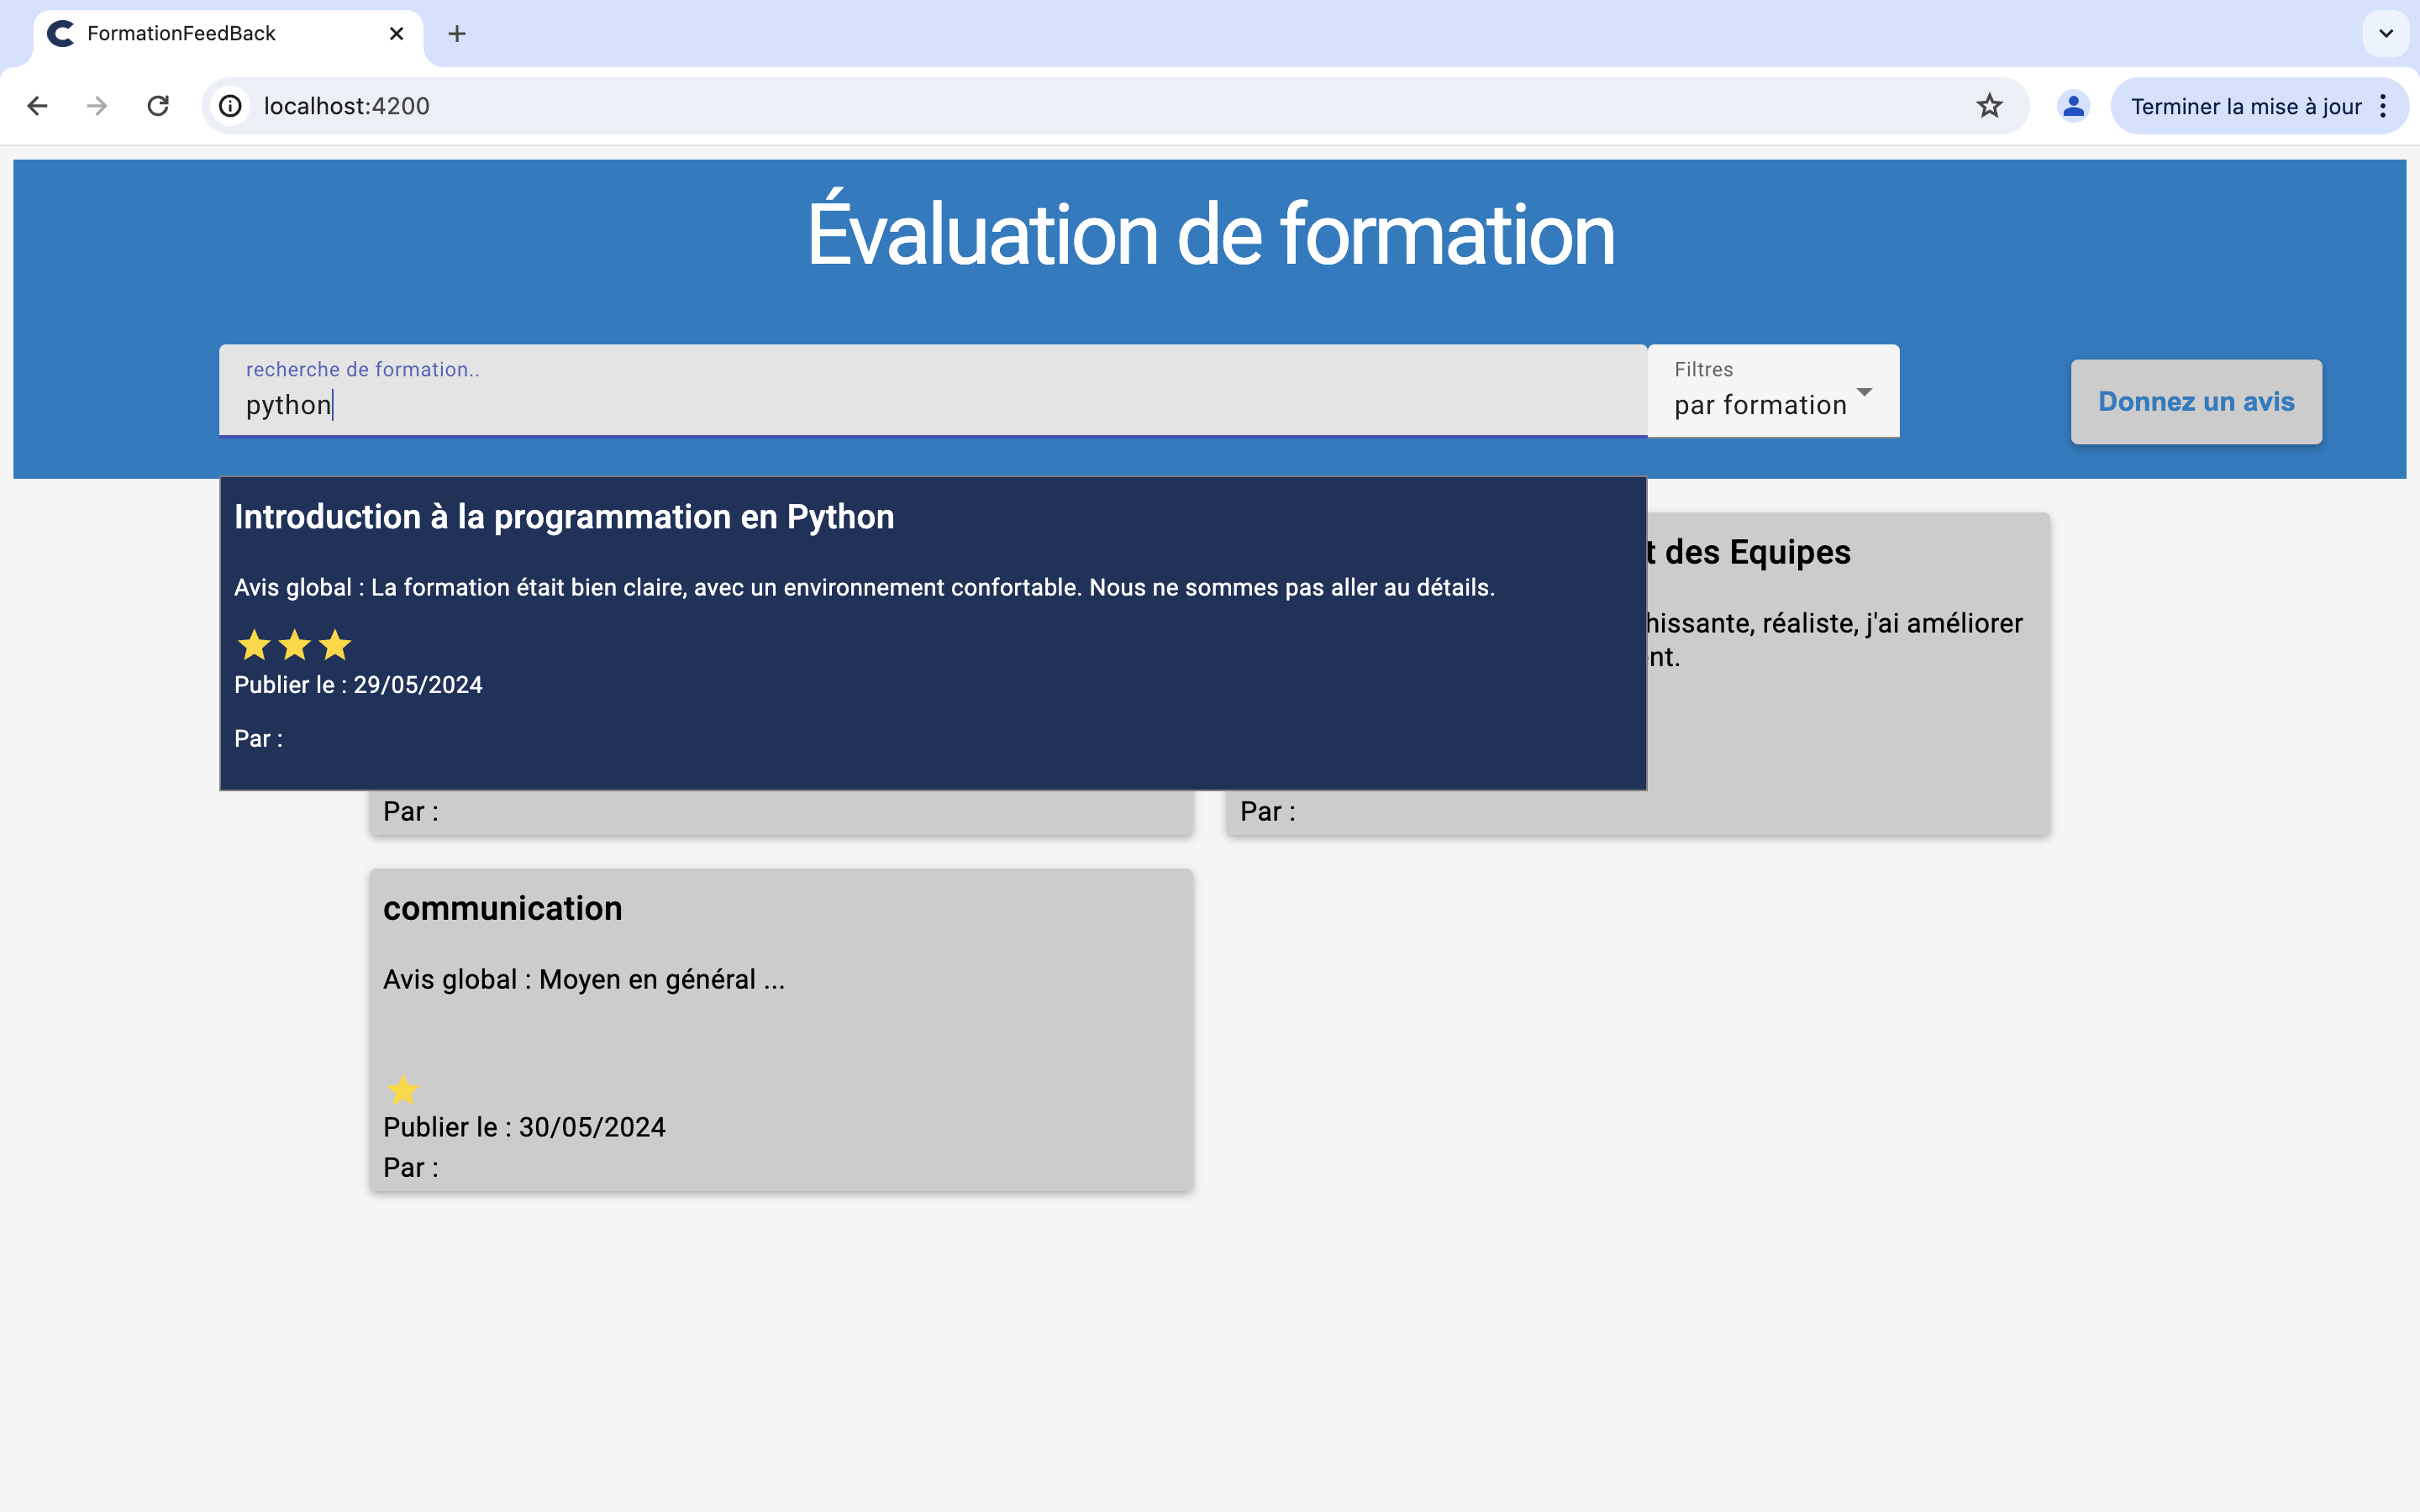
\includegraphics[width=1\textwidth]{images/fenetres/rechercheAvis.png}
    \caption{Rechercher un avis avec un mot clé}
\end{figure}

\newpage

\section*{Détails d'un avis}
L'agent peut consulter le détails d'un avis qu'il sélectionne.
\medskip

\begin{figure}[h!]
    \centering
    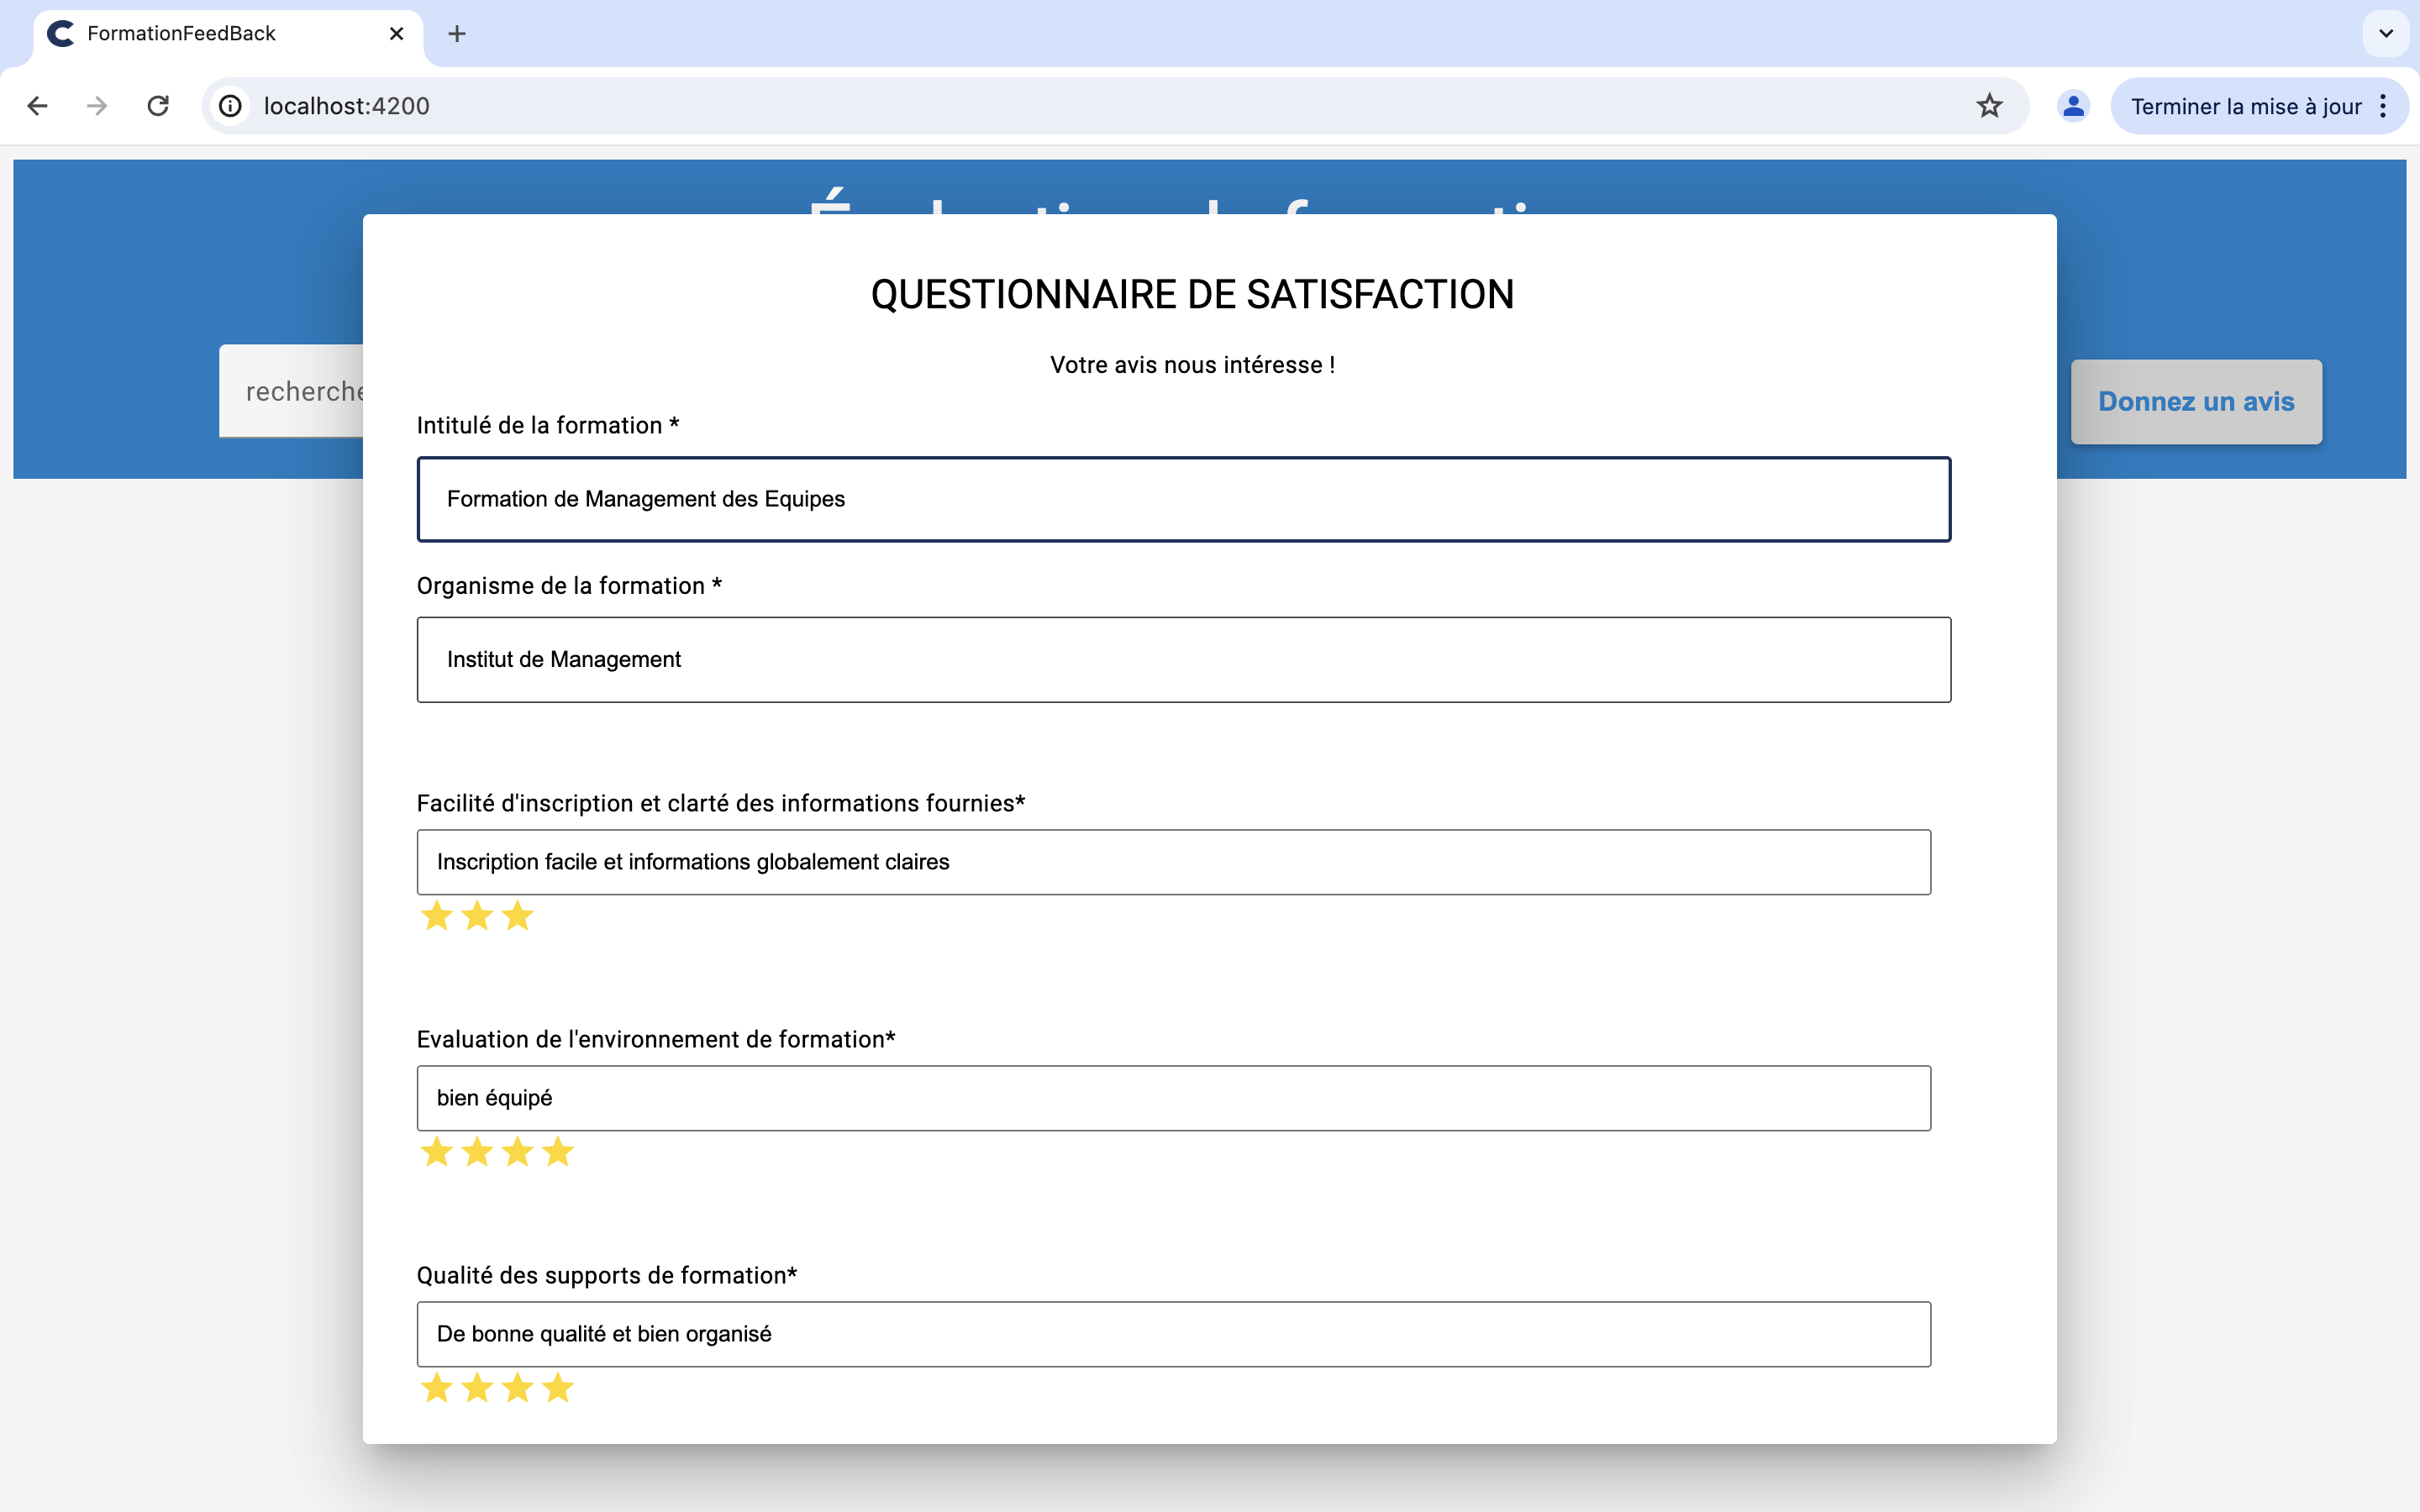
\includegraphics[width=1\textwidth]{images/fenetres/DetailsAvis.png}
    \caption{Détails d'un avis}
\end{figure}
\medskip